\documentclass[11pt]{article}
\usepackage{geometry}                
\geometry{letterpaper}                 
\usepackage[parfill]{parskip}        
\usepackage{graphicx}
\usepackage{amssymb}
\usepackage{amsmath}
\usepackage{epstopdf}
\usepackage{verbatim}
\usepackage{float}
\usepackage{enumerate}
\usepackage{hyperref}
\usepackage[utf8]{inputenc}
\usepackage[T1]{fontenc}
\DeclareGraphicsRule{.tif}{png}{.png}{`convert #1 `dirname #1`/`basename #1 .tif`.png}
\usepackage{color}
\usepackage{textcomp}
\definecolor{listinggray}{gray}{0.9}
\definecolor{lbcolor}{rgb}{1,1,1}

\begin{document}
{\small
\section*{Problems for Discussion 5, 10/23/13}
Compiled by Mai Le, some problems from Prof. Fessler, Prof. Yagle
}

\section{Alternative Sampling Theorem}
% Fessler 556, hmwk 3, p4

Generalize the ideal impulse sampling theory to the more realistic case to account for finite detector size:

\[
g_d[n] = \frac{1}{T}\int_{(n-\frac{1}{2})T}^{(n+\frac{1}{2})T} g_c(t) dt
\]

\section{Nyquist Rate for Communications Channel}
% Yagle Rec 2

A seismic signal with amplitude range [-1,1] volts is sampled and quantized with a 12 bit A/D converter before transmitting it over a communication channel which can support a maximum bit rate of 240 Kbits/sec. What is the maximum sampling frequency the system can support? What is the maximum frequency that can be present in the original seismic signal in order to avoid any loss of information?

\section{Sinc interpolation}
% Pradhan discussion
A signal x(t) has a triangular spectrum, with maximum frequencies $\pm \Omega_c$. x(t) is sampled at a rate of $f_s = \frac{1}{T_s}=\frac{\Omega_s}{2 \pi}$, producing the samples $\{x(nT_s)\}_{n=-\infty}^\infty$.

Let $y(t)$ be the signal constructed from these samples as follows:
\[
y(t) = \frac{ \Omega_c T_s}{\pi} \sum_{n=-\infty}^\infty x(nT_s) sinc\left( \frac{\Omega_c}{\pi} (t-nT_s) \right)
\]

How is $y(t)$ related to $x(t)$ when:

(a) $\Omega_c = \frac{\Omega_s}{4}$ 

(b) $\Omega_c = \Omega_s$?

\section{Relating CTFT and DTFT}
% Yagle Rec. 2

Suppose the CTFT of the continuous time signal $x_a(t)$ is as following.

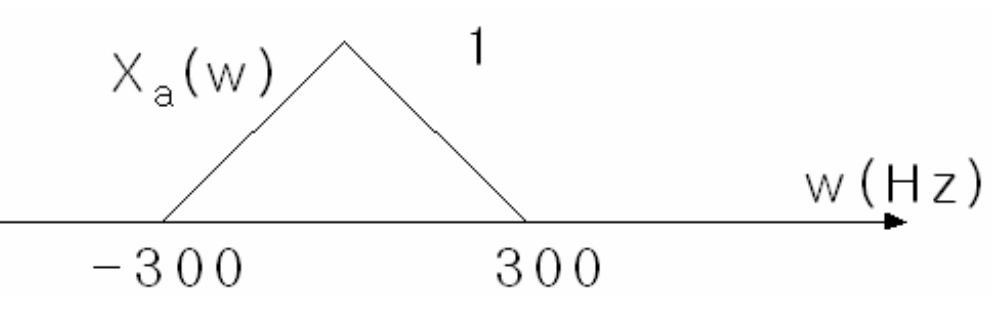
\includegraphics[width = 0.8\textwidth]{CTFT_p4.png} 

Determine the DTFT of the sampled signal $x[n]$, when the sampling period is 1 ms. What happens if the sampling period is 2 ms?
\end{document}